\documentclass{article}
\usepackage{arev}
\usepackage{tikz}
\usetikzlibrary{mindmap,arrows,decorations.pathmorphing,backgrounds,positioning,fit,petri}
\begin{document}

Experiments with points, nodes, and connections:
\tikz \draw (1,1) node[left] {one} -- (2,2) node[right] {two}  +(1,1) node[above,circle,draw] {two bis} -- ++(-1,1) node[above,rectangle,fill,color=yellow] {three} -- cycle ; 
Hmm, why does the yellow rectangle cover up the text?

Experiments with other paths: \tikz \fill[color=red] (0,0) rectangle (2, 1);.

\section{Experiment with trees}
\label{sec:exper-with-trees}
This is written in one line, and is hard to parse for me
\begin{center}
  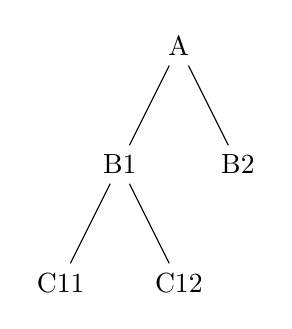
\begin{tikzpicture}
    \node {A} child {node {B1} child {node {C11}} child {node {C12}}} child {node {B2}} ;
  \end{tikzpicture}
\end{center}

Same thing but with indentation on multiple lines
\begin{center}
  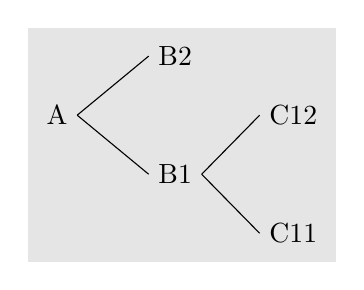
\begin{tikzpicture}
    [parent anchor=east, child anchor=west, grow=east, 
    every node/.style={ball,ball color=red,circle,text=white} 
    edge from parent/.style={draw,dashed,thick,red}] 
    \path
    node (A) {A} 
    child {
      node (B1) {B1} 
      child {node (C11) {C11}} 
      child {node (C12) {C12}}} 
    child {
      node (B2) {B2}} 
    ;
  \begin{pgfonlayer}{background} 
    \node [fill=black!10, fit=(A) (C11) (C12) (B2)] {}; 
  \end{pgfonlayer} 
  \end{tikzpicture}
\end{center}
The way to think of this is that \verb|child {SUBTREE}| makes a
sub-tree that buds from the current node, where \texttt{SUBTREE} must
be \verb|node {CONTENTS}| followed by zero or more \verb|child {SUBTREE}|. 

\section{Tests of background layer}
\label{sec:tests-backgr-layer}

The following need all these libraries to be laoded:
\begin{verbatim}
\usetikzlibrary{arrows,decorations.pathmorphing,backgrounds,positioning,fit,petri}
\end{verbatim}
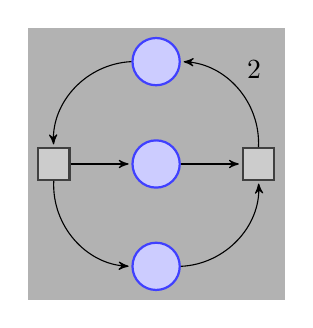
\begin{tikzpicture}
  [node distance=1.3cm,on grid,>=stealth',bend angle=45,auto, 
  every place/.style= {minimum size=6mm,thick,draw=blue!75,fill=blue!20}, 
  every transition/.style={thick,draw=black!75,fill=black!20}, 
  red place/.style= {place,draw=red!75,fill=red!20}, 
  every label/.style= {red}] 
  \node[place] (waiting) {}; 
  \node[place] (critical) [below=of waiting] {}; 
  \node[place] (semaphore) [below=of critical] {}; 
  \node[transition] (leave critical) [right=of critical] {} 
  edge [pre] (critical) 
  edge [post,bend right] node[auto,swap] {2} (waiting) 
  edge [pre, bend left] (semaphore); 
  \node[transition] (enter critical) [left=of critical] {} 
  edge [post] (critical) 
  edge [pre, bend left] (waiting) 
  edge [post,bend right] (semaphore); 
  \begin{pgfonlayer}{background} 
    \node [fill=black!30,fit=(waiting) (critical) (semaphore) 
    (leave critical) (enter critical)] {}; 
  \end{pgfonlayer} 
\end{tikzpicture} 

\section{Filling page with background image}
\label{sec:tests-filling-page}
\graphicspath{ {../figs/}, }
The cartoon is drawn on the background layer.\\
\begin{tikzpicture}
  [mybox/.style={fill=blue!50!black, semitransparent, text opacity=1, 
    text=green!30!white, shape=rectangle, inner sep=0.5cm}]
  \begin{pgfonlayer}{background} 
    \node (pic)
    {\includegraphics[width=\textwidth]{globule/Globule-Structure-New}} ;
  \end{pgfonlayer} 
  \node [mybox, node distance=0.5cm] (hello) 
  [below right=of pic.north west] {\huge \textbf{Hello \dots}} ; 
  \node [mybox] (goodbye) [below right=of hello] {\small \textbf{\dots
      and Goodbye}} ; 
  \node [mybox, text=yellow, node distance=0cm] (star) [above right=of goodbye]{\huge\textbf{\boldmath$\star$}} ; 
\end{tikzpicture}

\section{Background image with mindmap}
\label{sec:backgr-image-with}

\begin{tikzpicture}[mindmap,
  concept color=green!50!black, 
  fill opacity=0.8, draw opacity=0.0, text opacity=1,
  text=white,
  % inner sep=0cm, node distance=0cm,
  every annotation/.style={fill=red!20},
  ]
  \bfseries
  \path
  node[concept, concept color=green!50!black] (root) {Turbulent H\,II Regions} 
  child [concept color=blue!50!black, grow=south east] {node[concept] {Initial Conditions}
    child [concept color=red, grow=down] {node[concept, concept color=red] {Evolution}
    }
  }
  child [grow=south west] {
    node[concept] (globule) {Zoom on globule}
  }
  ;
  \begin{pgfonlayer}{background} 
    \node [node distance=0cm] (rgb-pic) [left=of globule.north east]
    {\includegraphics[width=0.6\paperwidth]{src/rgb-im-Bstar-mosaic-bright}} ;
  \end{pgfonlayer} 
  \begin{pgfonlayer}{background} 
    \node [node distance=0cm] (hsv-pic) [below=of rgb-pic.south]
    {\includegraphics[width=0.6\paperwidth]{src/mhdcuts-Bstar-mosaic-bright}} ;
  \end{pgfonlayer} 
  \begin{pgfonlayer}{background} 
    \node[annotation,below left,text width=5cm] (globule-image) at (globule.center) {
      \includegraphics[width=\linewidth]{globule/paper-emview-new}
    };
    \node[annotation,below right,text width=3cm] (globule-cartoon) at (globule-image.east) {
      \includegraphics[width=\linewidth]{globule/Globule-Structure-New}
    };
  \end{pgfonlayer}
\end{tikzpicture}

Test of color change: \tikz[mindmap,concept color=blue!80] 
\node [concept] {Root concept} 
child[concept color=red,grow=30] {node[concept] {Child concept}} 
child[concept color=orange,grow=0] {node[concept] {Child concept}}; 
This works fine, so why doesn't the above work?

\tikzset{
  wjh-concept/.style={
    concept, concept color=white!80!blue, text=black
  }}

\begin{tikzpicture}[huge mindmap]
 \path
  node[wjh-concept] {\huge\bfseries Turbulent H\,II Regions} 
  ;
  \begin{pgfonlayer}{background}
    \node {Hello};
    % \node {\includegraphics[width=\textwidth]{rgb-im-Bstar-mosaic-bright}};
  \end{pgfonlayer}

\end{tikzpicture} 

\section{Using tex dimensions}
\label{sec:using-tex-dimensions}

Result of \texttt{1in + 10pt} is \pgfmathparse{1in + 10pt} \pgfmathresult

Result of \verb|\paperwidth| is \pgfmathparse{\paperwidth} \pgfmathresult


\end{document}
